\documentclass[crop,tikz]{standalone}
\usepackage{tikz-3dplot}
\makeatletter
\usetikzlibrary{3d}
\begin{document}


% kepler_2_particles
\tdplotsetmaincoords{70}{110}
  \begin{tikzpicture}[scale=4, tdplot_main_coords]
  	
    \coordinate (O) at (0,0,0);
    \draw[thick] (-1.5,0,0) -- (O);
    \draw[thick] (0,-1,0) -- (O);
    \draw[thick] (0,0,-0.75) -- (O);
    \draw[->, >=latex, thick] (O) -- (1.5,0,0) node[anchor=north east, yshift=1mm]{$X$};
    \draw[->, >=latex, thick] (O) -- (0,1,0) node[right]{$Y$};
    \draw[->, >=latex, thick] (O) -- (0,0,0.75) node[left]{$Z$};
    
    % Define coordinates of the two bodies
    \pgfmathsetmacro{\px}{0.5};
    \pgfmathsetmacro{\py}{-0.9};
    \pgfmathsetmacro{\pz}{0.5};
    \pgfmathsetmacro{\dx}{-1};
    \pgfmathsetmacro{\dy}{0.8};
    \pgfmathsetmacro{\dz}{0.3};
    \coordinate (M1) at (\px,\py,\pz);
    \coordinate (M2) at (\dx,\dy,\dz);
    
    % Draw the bodies
    \fill[fill=blue!50!black!50] (M1) circle (1pt);
    \fill[fill=red!50!black!50] (M2) circle (1pt);
    
    % Draw the positions of each body relative to the origin
    \draw[->,>=stealth] (O) -- (M1) node[pos=0.7, above, yshift=1mm]{$\mathbf{r}_1$};
    \draw[->,>=stealth] (O) -- (M2) node[pos=0.7, above, yshift=1mm]{$\mathbf{r}_2$};
    
    % Draw the projections of both bodies onto the plane
    \draw[dashed] (M1) -- (\px, \py, 0);
    \draw[dashed] (\px, \py, 0) -- (0, \py, 0);
    \draw[dashed] (\px, \py, 0) -- (\px, 0, 0);
    \draw[dashed] (M2) -- (\dx, \dy, 0);
    \draw[dashed] (\dx, \dy, 0) -- (0, \dy, 0);
    \draw[dashed] (\dx, \dy, 0) -- (\dx, 0, 0);
    
    
    %% Draw the vector from body 1 to body 2
    %\draw[->,>=stealth] (M1) -- (M2) node[pos=0.6, above]{$\vec{r}$};
    
    % Provide the masses
    \node at (M1) [left, xshift=-0.75mm]{$m_1$};
    \node at (M2) [right, xshift=1mm]{$m_2$};
  \end{tikzpicture}

\newpage
% reduced_mass_system
\tdplotsetmaincoords{70}{110}
  \begin{tikzpicture}[scale=4, tdplot_main_coords]
	% Draw a sample trajectory that the particle takes
	\begin{scope}
		% Draw "rings" where the trajectory "passes through the horizontal plane"
		\foreach \t in {49.25, 149.4} {
			\pgfmathsetmacro{\x}{2-cos(\t)^2}
			\pgfmathsetmacro{\y}{-0.35*cos(\t)+\t/180}
			\pgfmathsetmacro{\z}{cos(\t)^2-0.1*sin(\t)}
			\begin{scope}[canvas is xy plane at z=\z]
				\draw[red!80!black!80] (\x,\y) circle (0.2 mm);
 			\end{scope}
 		}
 		
		% Define times at which the trajectory looks like it passes through
		% the planes
		\pgfmathsetmacro{\tlim}{105}
		\pgfmathsetmacro{\tlimTwo}{198}
		\pgfmathsetmacro{\tfinal}{255}
		
		% Flow from the reduced particle through the horizontal plane
		% up until passing through the vertical plane facing the screen
  		\begin{scope}[black, dashed, ->, >=stealth]
  			\pgfplothandlerlineto
  			\pgfplotfunction{\t}{0,1,...,\tlim}
       		{\pgfpointxyz {2-cos(\t)^2}{-0.35*cos(\t)+\t/180}{cos(\t)^2-0.1*sin(\t)}} 
       		\pgfusepath{stroke}
		\end{scope}
  		
  		% Flow in the background until coming back up front
  		\pgfmathsetmacro{\tlimPlusOne}{\tlim+1}
  		\pgfmathsetmacro{\tlimPlusTwo}{\tlim+2}
		\begin{scope}[black!40, dashed, ->, >=stealth]
  			\pgfplothandlerlineto
			\pgfplotfunction{\t}{\tlimPlusOne,\tlimPlusTwo,...,\tlimTwo}
       		{\pgfpointxyz {2-cos(\t)^2}{-0.35*cos(\t)+\t/180}{cos(\t)^2-0.1*sin(\t)}} 
       		\pgfusepath{stroke}
		\end{scope}
		
		% Finish the flow
    		\pgfmathsetmacro{\tlimTwoPlusOne}{\tlimTwo+1}
  		\pgfmathsetmacro{\tlimTwoPlusTwo}{\tlimTwo+2}
		\begin{scope}[black, dashed, ->, >=stealth]
  			\pgfplothandlerlineto
			\pgfplotfunction{\t}{\tlimTwoPlusOne,\tlimTwoPlusTwo,...,\tfinal}
       		{\pgfpointxyz {2-cos(\t)^2}{-0.35*cos(\t)+\t/180}{cos(\t)^2-0.1*sin(\t)}} 
       		\pgfusepath{stroke}
		\end{scope}
    \end{scope}
  
  	
    \coordinate (O) at (0,0,0);
    \draw[thick] (-1.5,0,0) -- (O);
    \draw[thick] (0,-1,0) -- (O);
    \draw[thick] (0,0,-0.725) -- (O);
    \draw[->, >=latex, thick] (O) -- (1.5,0,0) node[anchor=north east, yshift=1mm]{$X$};
    \draw[->, >=latex, thick] (O) -- (0,1.1,0) node[right]{$Y$};
    \draw[->, >=latex, thick] (O) -- (0,0,0.75) node[left]{$Z$};
  	
	% Define the position of the reduced mass particle
  	\coordinate (M) at (1,-0.35,1);
	
	% Draw the reduced mass body
    \fill[fill=green!50!black!50] (M) circle (0.5pt);
    
    % Draw the position of the reduced mass body relative to the other body
    \draw[->,>=stealth] (O) -- (M) node[pos=0.7, above, yshift=+1mm]{$\mathbf{r}$};
    
    % Draw the massive body
    \fill[fill=black!50] (O) circle (1pt);
    
    % Draw the anchor at the origin (mass m1 + m2) and the reduced mass particle
  	\node at (O) [anchor=north west, xshift=1mm, rotate=-6]{$m_1 + m_2$};
    \node at (M) [left]{$\mu^*$};
  \end{tikzpicture}

\newpage
% kepler_solution
  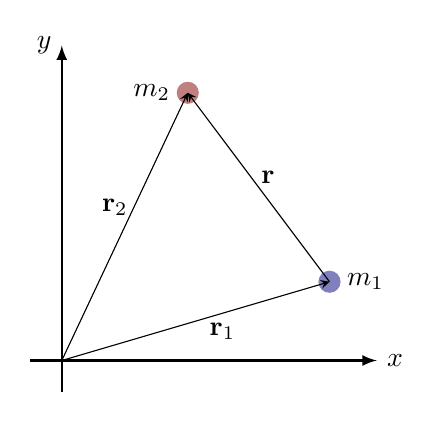
\begin{tikzpicture}[scale=4]
    \coordinate (O) at (0,0);
    \draw[thick] (-0.1,0) -- (O);
    \draw[thick] (0,-0.1) -- (O);
    \draw[->, >=latex, thick] (O) -- (1,0) node[right]{$x$};
    \draw[->, >=latex, thick] (O) -- (0,1) node[left]{$y$};
    
    % Define coordinates of the two bodies
    \pgfmathsetmacro{\px}{0.85};
    \pgfmathsetmacro{\py}{0.25};
    \pgfmathsetmacro{\dx}{0.4};
    \pgfmathsetmacro{\dy}{0.85};
    \coordinate (M1) at (\px,\py);
    \coordinate (M2) at (\dx,\dy);
    
    % Draw the bodies
    \fill[fill=blue!50!black!50] (M1) circle (1pt);
    \fill[fill=red!50!black!50] (M2) circle (1pt);
    
    % Draw the positions of each body relative to the origin
    \draw[->,>=stealth] (O) -- (M1) node[pos=0.6, below, yshift=0mm]{$\mathbf{r}_1$};
    \draw[->,>=stealth] (O) -- (M2) node[pos=0.6, left, yshift=-1mm]{$\mathbf{r}_2$};
    
    % Draw the vector from body 1 to body 2
    \draw[->,>=stealth] (M1) -- (M2) node[pos=0.55, right]{$\mathbf{r}$};
    
    % Provide the masses
    \node at (M1) [right, xshift=1mm]{$m_1$};
    \node at (M2) [left, xshift=-1mm]{$m_2$};
  \end{tikzpicture}

\newpage
% Kepler coordinate rotation
\tdplotsetmaincoords{70}{110}
  \begin{tikzpicture}[scale=4, tdplot_main_coords]
	% Define the position of the reduced mass particle
	\pgfmathsetmacro{\Mx}{-1}
	\pgfmathsetmacro{\My}{0.75}
	\pgfmathsetmacro{\Mz}{0}
	% Draw a sample trajectory that the particle takes
	\begin{scope}
		% Flow from the reduced particle through the horizontal plane
		% up until passing through the vertical plane facing the screen
  		\begin{scope}[black, dashed, ->, >=stealth]
  			\pgfplothandlerlineto
  			\pgfplotfunction{\t}{0,1,...,360}
       		{\pgfpointxyz {\Mx - sin(\t*2) + \t/180}{\My - 2*sin(\t/2)}{0}} 
       		\pgfusepath{stroke}
       		% Label the trajectory as planar
       		\node at (-1.1, -0.9){planar trajectory};
		\end{scope}
%  		
%  		% Flow in the background until coming back up front
%  		\pgfmathsetmacro{\tlimPlusOne}{\tlim+1}
%  		\pgfmathsetmacro{\tlimPlusTwo}{\tlim+2}
%		\begin{scope}[black!40, dashed, ->, >=stealth]
%  			\pgfplothandlerlineto
%			\pgfplotfunction{\t}{\tlimPlusOne,\tlimPlusTwo,...,\tlimTwo}
%       		{\pgfpointxyz {-0.35*cos(\t)+\t/180}{cos(\t)^2-0.1*sin(\t)}{2-cos(\t)^2}} 
%       		\pgfusepath{stroke}
%		\end{scope}
%		
%		% Finish the flow
%    		\pgfmathsetmacro{\tlimTwoPlusOne}{\tlimTwo+1}
%  		\pgfmathsetmacro{\tlimTwoPlusTwo}{\tlimTwo+2}
%		\begin{scope}[black, dashed, ->, >=stealth]
%  			\pgfplothandlerlineto
%			\pgfplotfunction{\t}{\tlimTwoPlusOne,\tlimTwoPlusTwo,...,\tfinal}
%       		{\pgfpointxyz {-0.35*cos(\t)+\t/180}{cos(\t)^2-0.1*sin(\t)}{2-cos(\t)^2}} 
%       		\pgfusepath{stroke}
%		\end{scope}
    \end{scope}

	\coordinate (O) at (0,0,0);
    \draw[thick] (-1.5,0,0) -- (O);
    \draw[thick] (0,-1,0) -- (O);
    \draw[thick] (0,0,-0.75) -- (O);
    \draw[->, >=latex, thick] (O) -- (1.5,0,0) node[anchor=north east, yshift=1mm]{$x$};
    \draw[->, >=latex, thick] (O) -- (0,1,0) node[right]{$y$};
    \draw[->, >=latex, thick] (O) -- (0,0,0.75) node[left]{$z$};
  	
	% Make coordinate for particle
  	\coordinate (M) at (\Mx, \My, \Mz);
	
	% Draw the (x, y) components
	\draw[dashed] (M) -- (\Mx, 0, 0);
	\draw[dashed] (M) -- (0, \My, 0);
	
    % Draw the position of the reduced mass body relative to the other body
    % with both r and t
    \draw (O) -- (M) node[pos=0.5, above, yshift=0mm]{$r$};
    % Draw the angle
    \tdplotdefinepoints(0,0,0)(0.5,0,0)(\Mx,\My,0)
	\tdplotdrawpolytopearc[->, >=stealth]{0.5}{anchor=north,xshift=-0mm, yshift=-0.5mm}{$\theta$}
    
	% Draw the reduced mass body
    \fill[fill=green!50!black!50] (M) circle (0.5pt);    
	% Draw the massive body
	\fill[fill=black!50] (O) circle (1pt);    
    
    % Draw the anchor at the origin (mass m1 + m2) and the reduced mass particle
  	\node at (O) [anchor=south east, xshift=-1mm, rotate=-6]{$m_1 + m_2$};
    \node at (M) [right]{$\mu^*$};
  \end{tikzpicture}

\newpage
% Kepler polar coordinates
\tdplotsetmaincoords{70}{110}
  \begin{tikzpicture}[scale=4, tdplot_main_coords]
  	
  \end{tikzpicture}

\end{document}